
\documentclass[10pt]{article}
\usepackage[utf8]{inputenc}
\usepackage{graphicx}
\usepackage{amsmath, amssymb}
\usepackage{geometry}
\usepackage{caption} 
\geometry{a4paper, margin=0.5in, landscape} 

\begin{document}

\section*{Comparative EIS Kinetics Report}
\textbf{Model Structure:} \texttt{R0-p(R1-p(R2,CPE2),CPE1)} \\
\textbf{Used data:} original data

\begin{center}
    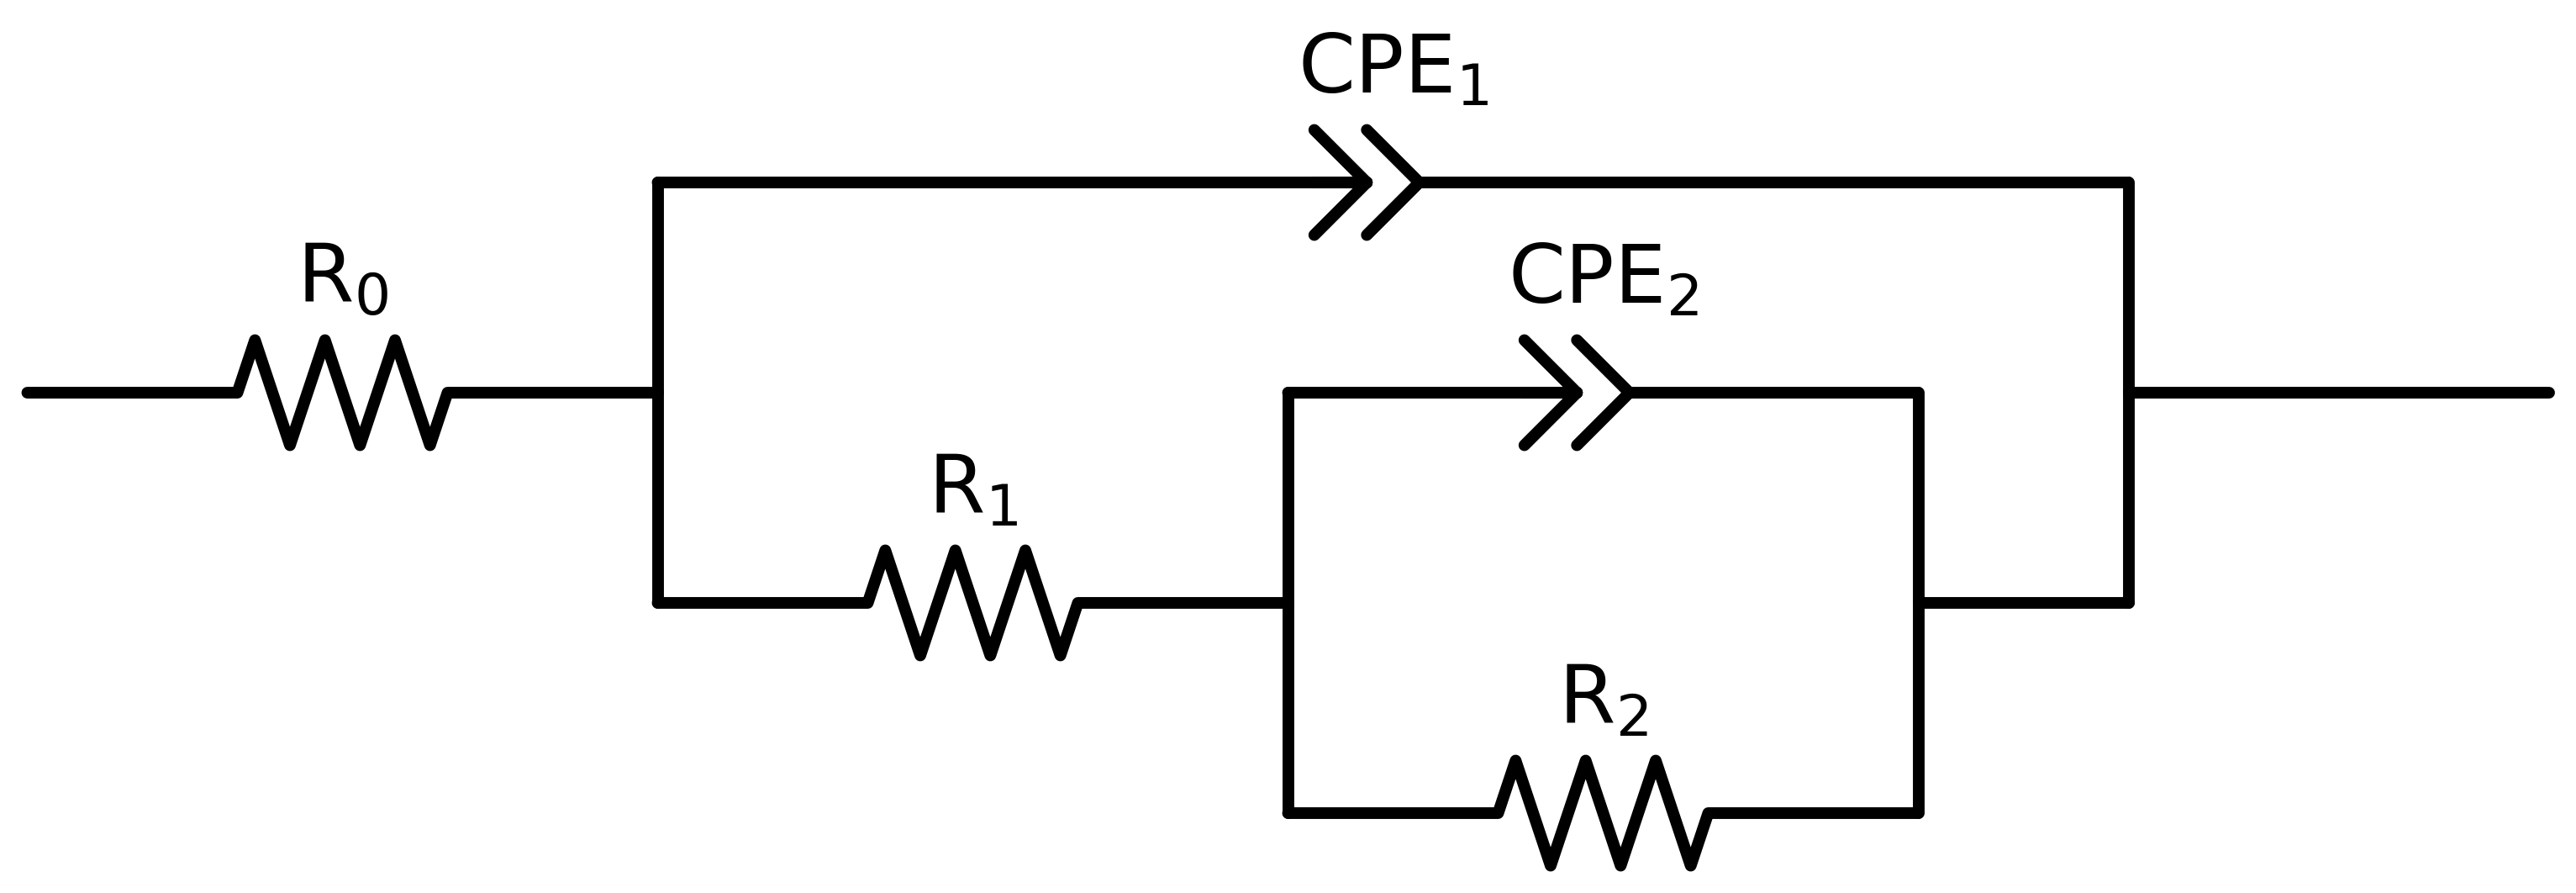
\includegraphics[width=0.45\textwidth]{../../../2RC.png}
\end{center}

\renewcommand{\arraystretch}{1.6} 
\begin{table}[h!]
    \centering
    \footnotesize
    \begin{tabular}{|l|c|c|c|c|c|}
        \hline
        \textbf{Element} & \textbf{Unit} & \textbf{Bounds} & \textbf{Cauvel\_4\_NaVO3\_1H} & \textbf{Cauvel\_4\_NaVO3\_4H} & \textbf{Cauvel\_4\_NaVO3\_8H} \\ \hline
        $R_{0}$ & $\Omega$ & $[1.0e-03, 1.0e+03]$ & $7.10e+01 \pm 8.7e-01$ & $6.50e+01 \pm 4.2e-01$ & $6.48e+01 \pm 3.1e-01$ \\ \hline
        $R_{1}$ & $\Omega$ & $[1.0e+00, 1.0e+08]$ & $2.48e+02 \pm 4.1e+02$ & $2.45e+05 \pm 6.8e+05$ & $3.01e+05 \pm 6.0e+03$ \\ \hline
        $R_{2}$ & $\Omega$ & $[1.0e+00, 1.0e+08]$ & $1.60e+05 \pm 2.5e+03$ & $1.40e+00 \pm 6.8e+05$ & $6.39e+04 \pm 3.0e+05$ \\ \hline
        $Q_{2}$ & $\Omega$$^{-1}$ sec$^{a}$ & $[1.0e-11, 1.0e-03]$ & $2.35e-06 \pm 5.5e-06$ & $4.77e-09 \pm 3.5e+05$ & $1.00e-03 \pm 2.1e-03$ \\ \hline
        $n_{2}$ & - & $[5.0e-01, 1.0e+00]$ & $9.03e-01 \pm 1.9e-01$ & $8.52e-01 \pm 6.8e-10$ & $1.00e+00 \pm 7.6e-01$ \\ \hline
        $Q_{1}$ & $\Omega$$^{-1}$ sec$^{a}$ & $[1.0e-11, 1.0e-03]$ & $5.56e-06 \pm 5.5e-06$ & $9.26e-06 \pm 1.1e-05$ & $9.58e-06 \pm 6.3e-08$ \\ \hline
        $n_{1}$ & - & $[5.0e-01, 1.0e+00]$ & $9.18e-01 \pm 9.3e-02$ & $8.77e-01 \pm 2.8e-02$ & $8.68e-01 \pm 1.3e-03$ \\ \hline
        \textbf{$\chi^2$} & - & -  & $1.538e-03$ & $7.052e-04$ & $4.486e-04$ \\ \hline

    \end{tabular}
\end{table}


\newpage
\section*{Analysis Results: 1H}
\begin{center}
    
\includegraphics[width=0.7\textwidth]{plots_Cauvel_4_NaVO3_1H_2RC.pdf}
    \captionof{figure}{EIS Fit Results for Cauvel\_4\_NaVO3\_1H}
\end{center}

\newpage
\section*{Analysis Results: 4H}
\begin{center}
    
\includegraphics[width=0.7\textwidth]{plots_Cauvel_4_NaVO3_4H_2RC.pdf}
    \captionof{figure}{EIS Fit Results for Cauvel\_4\_NaVO3\_4H}
\end{center}

\newpage
\section*{Analysis Results: 8H}
\begin{center}
    
\includegraphics[width=0.7\textwidth]{plots_Cauvel_4_NaVO3_8H_2RC.pdf}
    \captionof{figure}{EIS Fit Results for Cauvel\_4\_NaVO3\_8H}
\end{center}


\end{document}
